% LuaLaTeX + jlreq
% ビルド: latexmk -lualatex paper.tex
\documentclass[paper=a4,fontsize=10pt]{jlreq}

\usepackage{amsmath,amssymb}
\usepackage{graphicx}
\usepackage{booktabs}
\usepackage{array}
\usepackage{longtable}
\usepackage{capt-of}
\usepackage{xcolor}
\usepackage{listings}
\usepackage{tikz}
\usetikzlibrary{positioning,arrows.meta}
\usepackage{flafter}
\usepackage[haranoaji]{luatexja-preset}
\usepackage{xurl}
\usepackage[hidelinks,pdfusetitle]{hyperref}

% 図表を本文の近くに置き，図表だけのページを減らす
\renewcommand{\topfraction}{0.9}
\renewcommand{\bottomfraction}{0.8}
\renewcommand{\textfraction}{0.08}
\renewcommand{\floatpagefraction}{0.8}
\setcounter{topnumber}{3}
\setcounter{totalnumber}{4}
% 図表と本文の間隔（jlreq の既定は行間1つぶんで詰まって見えるため広げる）
\setlength{\textfloatsep}{1.5\baselineskip plus 0.5\baselineskip minus 0.2\baselineskip}
\setlength{\intextsep}{1.3\baselineskip plus 0.4\baselineskip minus 0.2\baselineskip}
\setlength{\floatsep}{1.3\baselineskip plus 0.4\baselineskip minus 0.2\baselineskip}
% 表の見出しと上の罫線の間隔
\setlength{\abovetopsep}{4pt}
% フロートにしない表：前後に本文との間隔をとり，見出しと本体を同じページに保つ
\newenvironment{heretable}
  {\par\addvspace{\intextsep}\noindent\begin{minipage}{\linewidth}\centering}
  {\end{minipage}\par\addvspace{\intextsep}}

\lstset{
  basicstyle=\ttfamily\small,
  columns=fullflexible,
  keepspaces=true,
  breaklines=true,
  frame=single,
  framesep=4pt,
  rulecolor=\color{black!30},
  xleftmargin=1\zw,
  xrightmargin=1\zw,
  aboveskip=\medskipamount,
  belowskip=\medskipamount
}

% 表の本体を読み込む（tabular 内で \input の直後に罫線を置けるようプリミティブを使う）
\makeatletter
\newcommand{\tabinput}[1]{\@@input #1 }
\makeatother
\newcommand{\code}[1]{\texttt{#1}}
\newcommand{\man}{\,万円}

\title{日本の国民負担率インタラクティブダッシュボード\\
  --- データ，仕組み，公開方法と生成AIによる開発過程 ---}
\author{河合勝彦\thanks{名古屋市立大学大学院経済学研究科．
  E-mail: \texttt{kkawai@econ.nagoya-cu.ac.jp}}}
\date{2026年10月4日}

\begin{document}
\maketitle

\begin{abstract}
本稿は，日本の国民負担率（租税負担率と社会保障負担率の合計）を可視化するウェブアプリ
「日本の国民負担率インタラクティブダッシュボード」の解説である。
本アプリは，財務省が公表する1970〜2026年度の国民負担率の推移，税目別の内訳，
OECD加盟35カ国との国際比較を図表で示し，あわせて給与所得者の所得税・住民税・社会保険料を
令和8（2026）年の制度で概算するシミュレーターを備える。
実装はビルドを要しない単一のHTMLファイルで，GitHub Pages と Cloudflare Workers から静的に配信している。
開発では，Gemini 3.8 Flash が生成したプロトタイプを，Claude Fable 5.1 が一次資料と照合して修正・拡充した。
プロトタイプは画面の体裁こそ整っていたが，推移データ13年度ぶんのうち内訳まで公式値と一致する年度は一つもなく，
国民負担率の合計も最大で5.0ポイントずれていた。
本稿では，指標の定義と読み方，データの出所，アプリの構成と計算モデル，公開の手順，
二つのモデルによる開発と検証の過程，限界および拡張の構想を記す。
\end{abstract}

\noindent
\textbf{キーワード}：国民負担率，租税負担率，社会保障負担率，潜在的国民負担率，
データ可視化，GitHub Pages，生成AI\\
\textbf{公開URL}：\url{https://katzkawai.org/kklab-tax-burden/}（GitHub Pages），
\url{https://kklab-tax-burden.katzkawai.workers.dev}（Cloudflare Workers）\\
\textbf{ソースコード}：\url{https://github.com/katzkawai/kklab-tax-burden}

\setcounter{tocdepth}{2}
\tableofcontents
\clearpage

\section{はじめに}

国民負担率は，税と社会保険料の負担が国民所得に対してどれだけの大きさかを示す指標で，
財務省が毎年公表している。令和8（2026）年度の見通しは45.7\%である\cite{mof2026}。
この数字は「所得のおよそ半分が税と保険料に消える」という意味で受け取られやすい。
しかし国民負担率は国全体を集計したマクロ指標であり，個人の給与から差し引かれる割合とは別のものである。
分子には法人が納める税や消費税，社会保険料の事業主負担分が含まれ，
分母の国民所得は国内総生産（GDP）より3割近く小さい。
同じ負担を対GDP比で測れば32.7\%になる。

本アプリの目的は，この指標の水準・推移・内訳・国際的な位置を一つの画面で確認できるようにし，
あわせて個人の負担を別に計算して見せることで，マクロ指標と個人の負担の違いを具体的に示すことにある。
授業や一般向けの説明で，その場で数値を確かめながら使うことを想定している。

本稿が記録するのは次の三点である。
\begin{enumerate}
  \item 国民負担率の定義，分母の違い，個人の負担との関係の整理（第\ref{sec:indicator}節）。
  \item 公表値だけを用いた可視化アプリの構成と，それを誰でも再現できる公開の手順
    （第\ref{sec:app}〜\ref{sec:hosting}節，付録\ref{app:cloudflare}）。
  \item 生成AIが作ったプロトタイプを別の生成AIが一次資料と照合して直した過程と，そこで見つかった誤りの内容
    （第\ref{sec:ai}・\ref{sec:verify}節）。
\end{enumerate}

本稿の構成は次のとおりである。
第\ref{sec:indicator}節で指標の定義と読み方を整理し，第\ref{sec:app}節でアプリの機能を，
第\ref{sec:data}節でデータとその出所を説明する。
第\ref{sec:impl}節で実装とシミュレーターの計算モデルを，第\ref{sec:hosting}節で公開と運用の方法を述べる。
第\ref{sec:ai}節は Gemini 3.8 Flash と Claude Fable 5.1 による開発過程，第\ref{sec:verify}節は検証である。
第\ref{sec:limits}節で限界を，第\ref{sec:extension}節で拡張の構想を述べる。
付録には，年度別データ，国際比較データ，Cloudflare Workers へのデプロイの詳細を収めた。

\section{国民負担率という指標}\label{sec:indicator}

\subsection{定義}

租税負担（国税と地方税の合計）を $T$，社会保障負担を $S$，国および地方の財政赤字を $D$，
国民所得を $\mathit{NI}$ とすると，財務省の定義は次のとおりである\cite{mof2026,mofa04}。
\begin{align}
  \text{国民負担率} &= \frac{T+S}{\mathit{NI}}\times 100
    = \underbrace{\frac{T}{\mathit{NI}}\times 100}_{\text{租税負担率}}
    + \underbrace{\frac{S}{\mathit{NI}}\times 100}_{\text{社会保障負担率}}, \label{eq:burden}\\
  \text{潜在的国民負担率} &= \frac{T+S+D}{\mathit{NI}}\times 100. \label{eq:potential}
\end{align}
潜在的国民負担率は，財政赤字を将来世代に先送りされた負担とみなして加えたものである。
加えるのは国債残高（ストック）ではなく，その年度の赤字（フロー）である。

\subsection{分母の違い}

国民所得（要素費用表示）とGDPの関係は
\begin{equation}
  \mathit{NI} = \mathit{GDP} + \text{海外からの所得の純受取} - \text{固定資本減耗}
     - (\text{生産・輸入品に課される税} - \text{補助金})
\end{equation}
である\footnote{支出側のGDPから求める場合は，このほかに統計上の不突合を差し引く。}。
固定資本減耗と間接税（純）を除くため，国民所得はGDPより小さい。
令和8年度見通しでは $\mathit{NI}/\mathit{GDP}=496.1/691.9\approx 0.717$ である。
対国民所得比の値を $b^{\mathit{NI}}$ とすると，対GDP比は
$b^{\mathit{GDP}} = b^{\mathit{NI}}\times \mathit{NI}/\mathit{GDP}$ で求まり，
45.7\%は32.7\%に対応する。
この比は一定ではない。財務省の表から計算すると，1970年度は0.81，1990年度は0.77，2010年度は0.71で，
対国民所得比と対GDP比の開きは長期的に広がってきた。
分子には消費税などの間接税が入るのに分母からは除かれるので，
間接税の比重が大きい国ほど対国民所得比は高く出やすい。
国際比較では両方の比率を見る必要がある。

\subsection{読むときの注意}

国民負担率を個人の負担率として読むのは，次の三点で適切でない。
\begin{enumerate}
  \item 分子には，個人が給与から直接支払わない負担が含まれる。
    令和8年度見通しの45.7\%のうち，法人所得課税が7.1\%，消費課税が8.8\%を占める（表\ref{tab:breakdown}）。
    社会保障負担17.6\%には事業主負担分が含まれる。
  \item 分母の国民所得には，雇用者報酬だけでなく企業所得と財産所得が含まれる。
  \item 負担した税と保険料は，年金・医療・介護などの給付や公共サービスとして国民に戻る。
    負担率だけでは受益の大きさは分からない。
\end{enumerate}
したがって，$100\%$ から国民負担率を引いた値を「国民の手取り」と呼ぶことはできない。
第\ref{sec:ai}節で述べるように，プロトタイプはこの読み方をグラフにしていた。

\begin{table}[htbp]
  \centering
  \caption{国民負担率の内訳（令和8年度見通し，対国民所得比）}\label{tab:breakdown}
  \begin{tabular}{llr}
    \toprule
    区分 & 主な税目など & 比率（\%）\\
    \midrule
    個人所得課税 & 所得税，個人住民税など & 8.5 \\
    法人所得課税 & 法人税，法人住民税，法人事業税など & 7.1 \\
    消費課税 & 消費税，酒税，揮発油税など & 8.8 \\
    資産課税等 & 固定資産税，相続税など & 3.6 \\
    \midrule
    租税負担率 & 国税 18.1 ＋ 地方税 9.9 & 28.0 \\
    社会保障負担率 & 社会保険料（本人負担＋事業主負担） & 17.6 \\
    \midrule
    国民負担率 & & 45.7 \\
    財政赤字 & & 2.7 \\
    潜在的国民負担率 & & 48.4 \\
    \bottomrule
  \end{tabular}

  \smallskip
  {\footnotesize 出所：財務省\cite{mof2026,mofa04}。四捨五入のため内訳の和は合計と一致しないことがある。}
\end{table}

\section{アプリの概要}\label{sec:app}

本アプリは一つのページからなり，上から順に次の七つの部分で構成される。

\begin{description}
  \item[最新指標] 国民負担率，租税負担率，社会保障負担率，潜在的国民負担率の最新値を4枚のカードで示す。
    国税・地方税の内訳，前年度比，対GDP比を添える。
  \item[推移グラフ] 1970〜2026年度の全57年度について，国税・地方税・社会保障負担を積み上げ棒で，
    潜在的国民負担率と対GDP比の国民負担率を折れ線で示す。
    表示期間は全期間，1990年度以降，2010年度以降の三つから選べる。
    実績見込みと見通しの年度は棒を淡色にして実績と区別する（図\ref{fig:overview}）。
  \item[内訳] 最新年度の国民負担率を，税の種類別と社会保障負担に分けて横棒で示す。
  \item[国際比較] OECD加盟35カ国の2023年の国民負担率を横棒で並べ，日本の行を強調する。
    対国民所得比と対GDP比を切り替えると，順位が入れ替わる様子を確認できる（図\ref{fig:intl}）。
    主要6カ国の潜在的国民負担率の表も付ける。
  \item[解説] 分母の違い，上昇の主因，潜在的国民負担率の意味，個人の負担との違いの4点を文章で説明する。
  \item[シミュレーター] 額面年収，配偶者控除の有無，扶養親族の人数，年齢区分を入力すると，
    所得税・住民税・社会保険料と手取り額を概算する（図\ref{fig:sim}）。
    国全体の社会保障負担率に含まれる事業主負担分も参考として表示する。
  \item[データ表] グラフの元データを年度別の表で示す。同じ内容をCSVファイルとして保存できる。
\end{description}

このほか，シミュレーターの入力条件をURLに含めて共有する機能がある。
画面幅に応じてレイアウトが変わり，スマートフォンでも閲覧できる。

\begin{figure}[tbp]
  \centering
  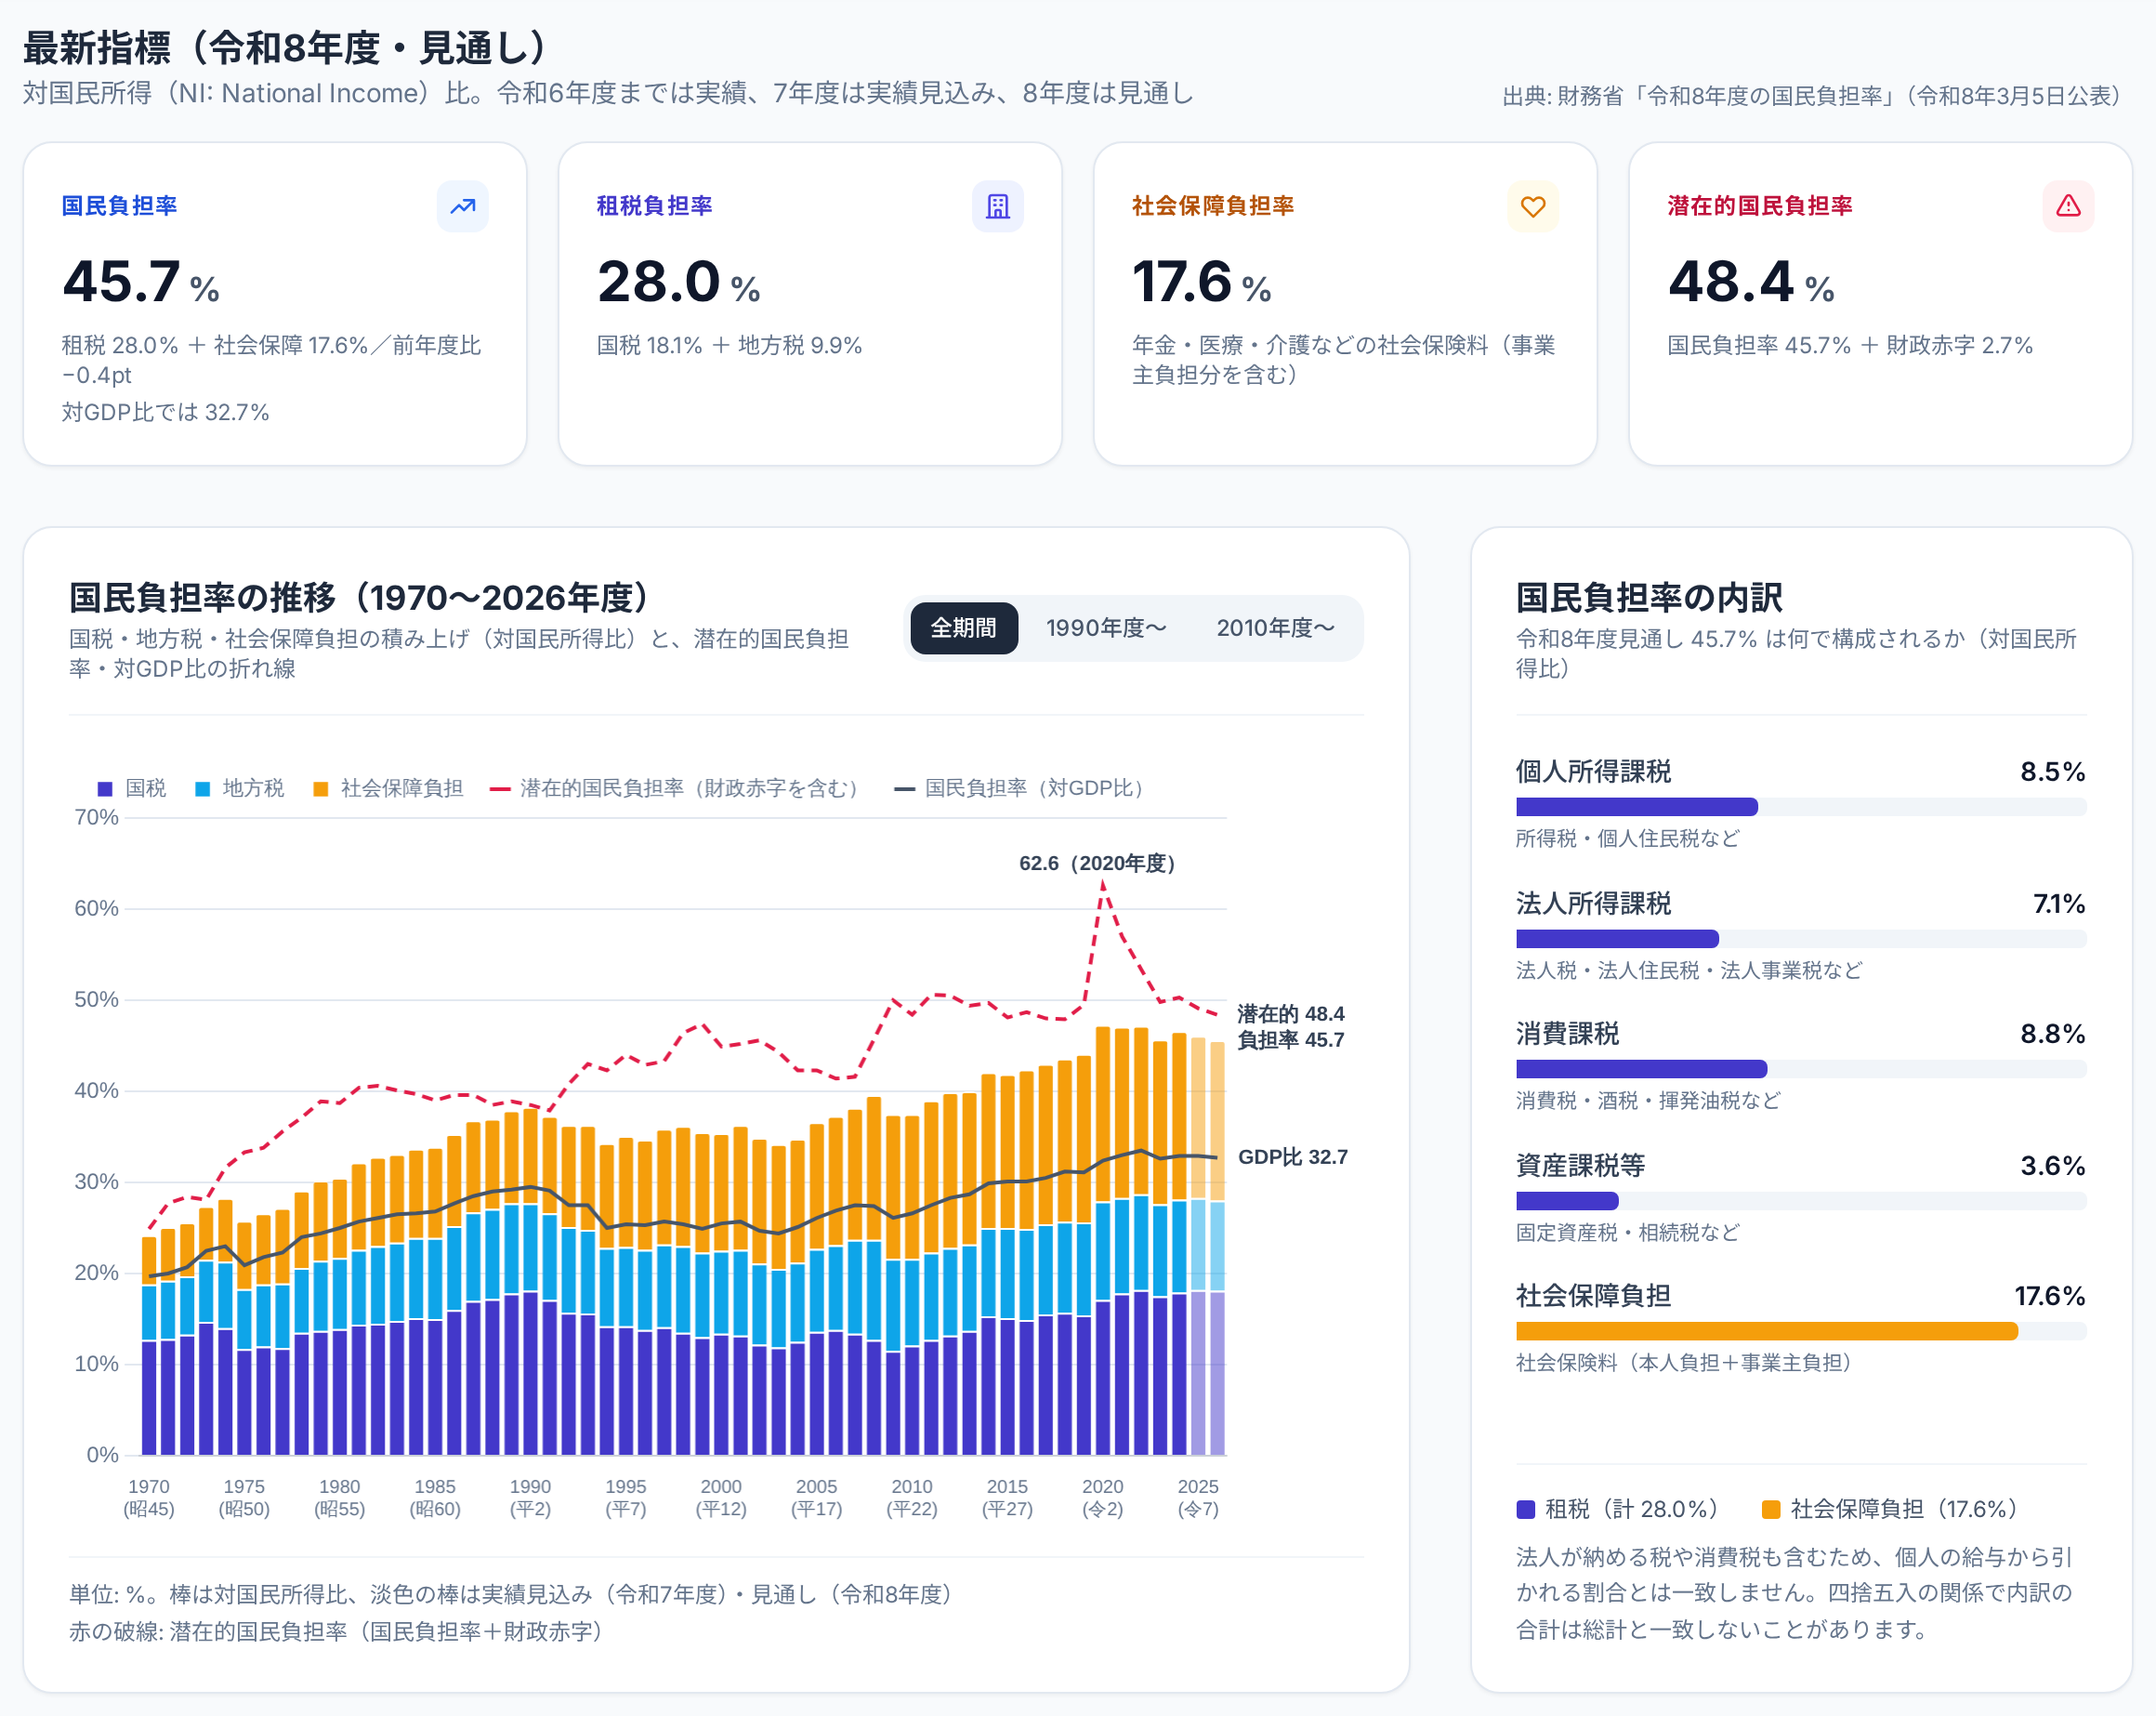
\includegraphics[width=\linewidth]{figures/fig_overview.png}
  \caption{最新指標のカード，推移グラフ，内訳}\label{fig:overview}
\end{figure}

\begin{figure}[tbp]
  \centering
  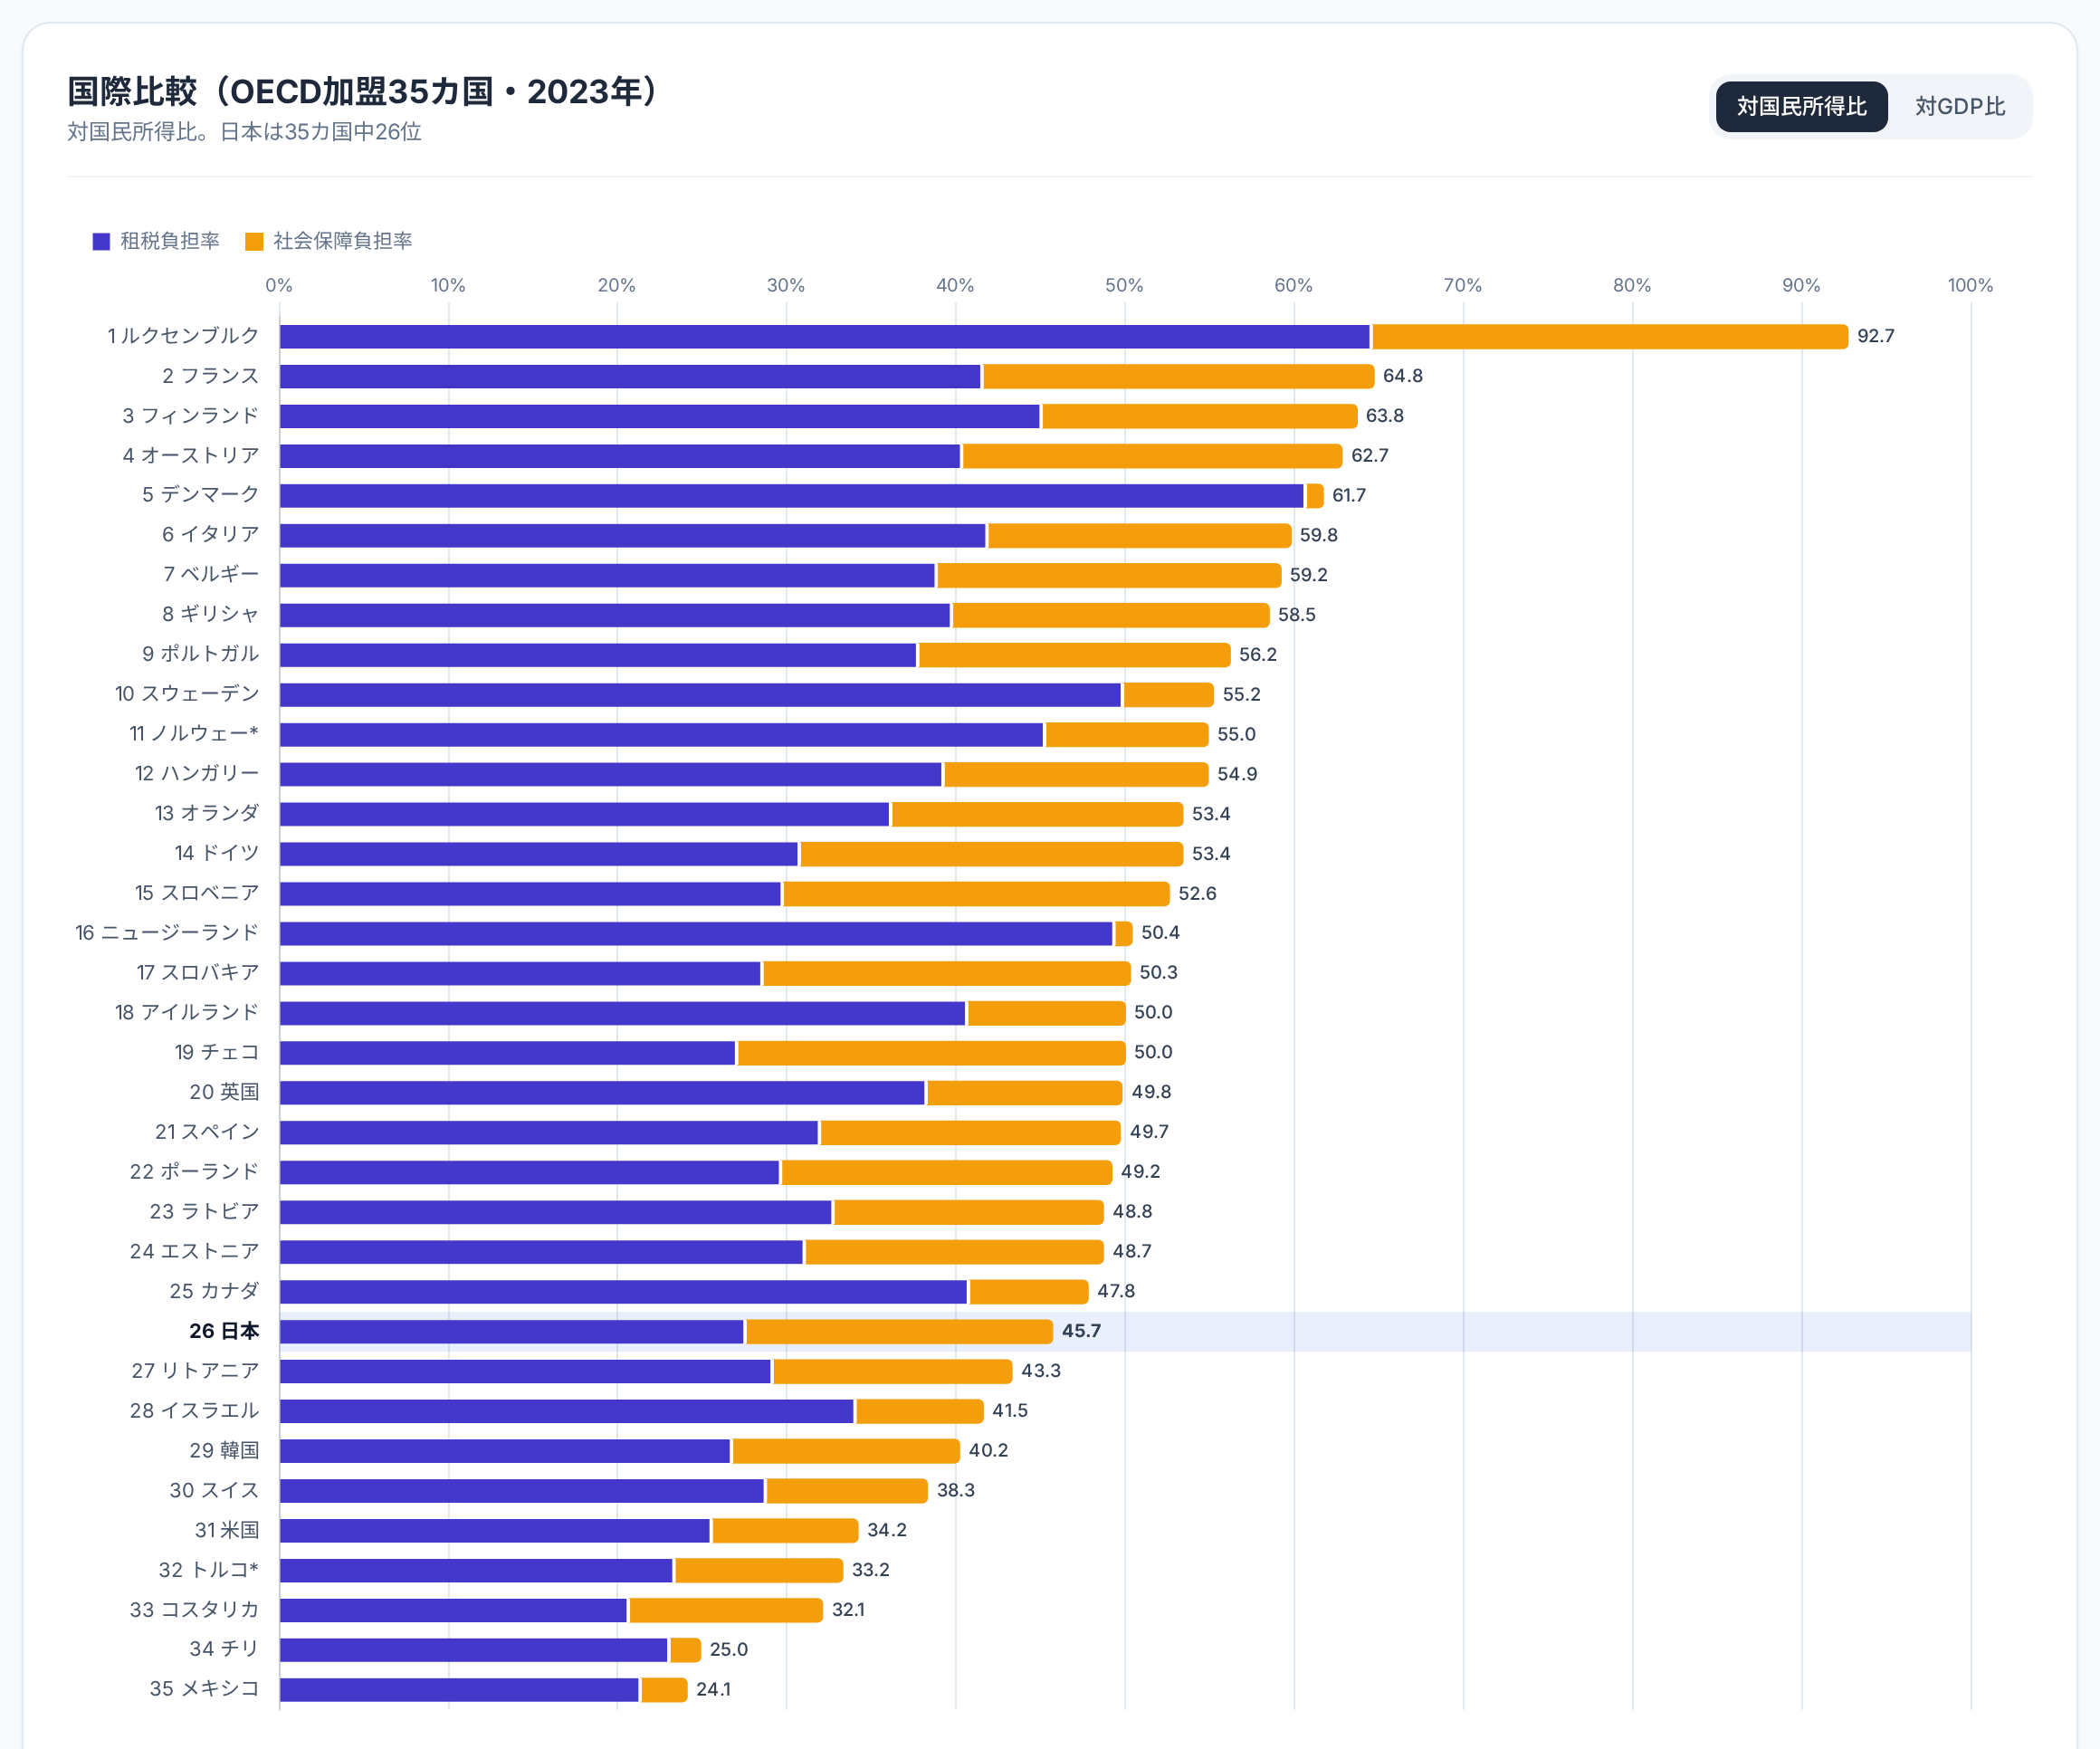
\includegraphics[width=0.92\linewidth]{figures/fig_intl.png}
  \caption{国際比較（OECD加盟35カ国，2023年，対国民所得比）}\label{fig:intl}
\end{figure}

\begin{figure}[tbp]
  \centering
  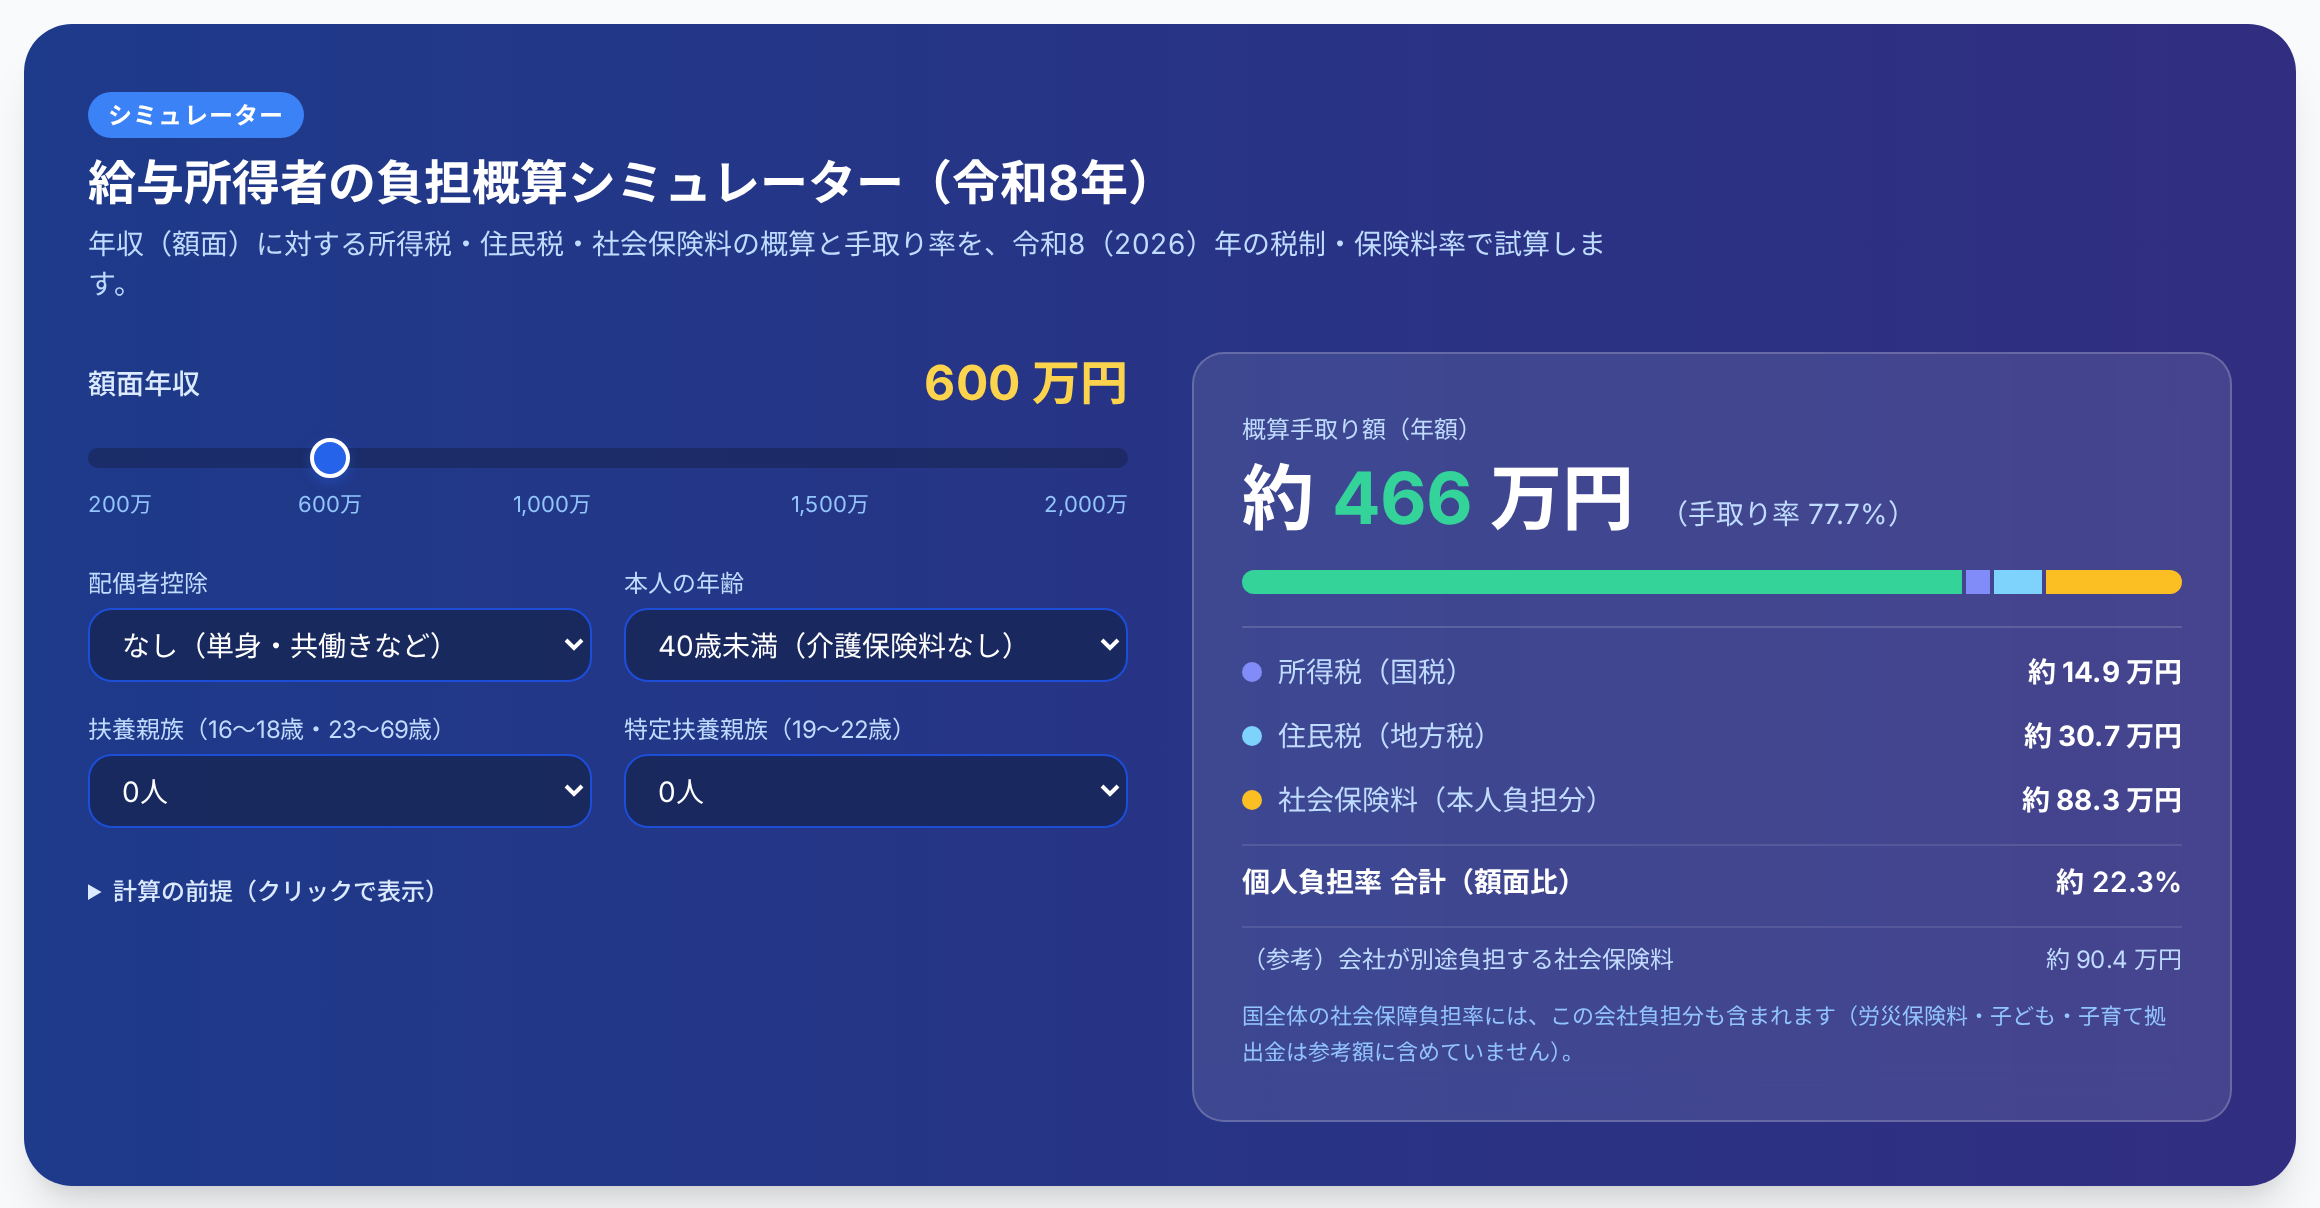
\includegraphics[width=\linewidth]{figures/fig_simulator.png}
  \caption{給与所得者の負担概算シミュレーター（年収600\man，単身，40歳未満の例）}\label{fig:sim}
\end{figure}

\section{データとその出所}\label{sec:data}

\subsection{出所の一覧}

アプリが用いる数値は，すべて公的機関の公表資料から転記したものである（表\ref{tab:sources}）。
独自の推計値は，シミュレーターの計算結果だけである。

\begin{table}[htbp]
  \centering
  \caption{データの出所}\label{tab:sources}
  \begin{tabular}{p{0.30\linewidth}p{0.62\linewidth}}
    \toprule
    内容 & 出所 \\
    \midrule
    国民負担率の推移（1970〜2026年度，10系列） &
      財務省「令和8年度の国民負担率を公表します」（2026年3月5日）の資料「国民負担率（対国民所得比）の推移」\cite{mof2026} \\
    国際比較（35カ国，主要6カ国） &
      同上の資料「国民負担率の国際比較」「国民負担率の国際比較（OECD加盟35カ国）」\cite{mof2026} \\
    租税負担率の税目別内訳 &
      財務省「負担率に関する資料」の「国民負担率及び租税負担率の推移（対国民所得比）」\cite{mofa04} \\
    所得税の控除額と税率 &
      国税庁「タックスアンサー」\cite{nta}，財務省「令和8年度税制改正の大綱」\cite{taikou2026} \\
    住民税の税率・均等割・調整控除 &
      総務省「個人住民税」\cite{soumu}，大綱\cite{taikou2026}，大阪市の解説\cite{osaka} \\
    健康保険・介護保険・子ども・子育て支援金の料率 &
      全国健康保険協会「令和8年度保険料率」\cite{kenpo2026} \\
    厚生年金の料率と標準報酬月額の上限 &
      日本年金機構「厚生年金保険の保険料」\cite{nenkin} \\
    雇用保険料率 &
      厚生労働省「令和8（2026）年度 雇用保険料率のご案内」\cite{mhlw2026} \\
    \bottomrule
  \end{tabular}
\end{table}

\subsection{推移データ}

推移データは，年度ごとに国税，地方税，租税負担率，社会保障負担率，国民負担率，財政赤字，
潜在的国民負担率，国民負担率の対GDP比，国民所得，GDPの10個の値を持つ。
財務省の表にはこのほか国税のうち一般会計税収の列があるが，アプリには収録していない。
全年度の値を付録\ref{app:trend}に掲げる。主な年度を抜き出すと表\ref{tab:selected}のとおりである。

\begin{table}[htbp]
  \centering
  \caption{国民負担率の推移（主な年度，\%）}\label{tab:selected}
  \begin{tabular}{lrrrrrr}
    \toprule
    年度 & 租税 & 社会保障 & 国民負担率 & 財政赤字 & 潜在的 & 対GDP比 \\
    \midrule
    1970（昭45） & 18.9 & 5.4 & 24.3 & 0.5 & 24.9 & 19.7 \\
    1980（昭55） & 21.7 & 8.8 & 30.5 & 8.2 & 38.7 & 25.0 \\
    1990（平2） & 27.7 & 10.6 & 38.4 & 0.1 & 38.5 & 29.5 \\
    2000（平12） & 22.5 & 12.9 & 35.4 & 9.5 & 44.9 & 25.5 \\
    2010（平22） & 21.5 & 15.9 & 37.4 & 11.0 & 48.4 & 26.6 \\
    2020（令2） & 27.9 & 19.4 & 47.3 & 15.3 & 62.6 & 32.4 \\
    2024（令6，実績） & 28.2 & 18.5 & 46.7 & 3.6 & 50.3 & 32.9 \\
    2025（令7，実績見込み） & 28.3 & 17.8 & 46.1 & 3.0 & 49.1 & 32.9 \\
    2026（令8，見通し） & 28.0 & 17.6 & 45.7 & 2.7 & 48.4 & 32.7 \\
    \bottomrule
  \end{tabular}

  \smallskip
  {\footnotesize 出所：財務省\cite{mof2026}。対GDP比を除き対国民所得比。}
\end{table}

この系列から読み取れる特徴を四つ挙げる。
\begin{itemize}
  \item \textbf{長期の上昇}：1980年度から2026年度見通しまでに国民負担率は30.5\%から45.7\%へ約15ポイント上昇した。
    このうち社会保障負担率が8.8\%から17.6\%へ8.8ポイント，租税負担率が21.7\%から28.0\%へ6.3ポイント上がっており，
    上昇の過半は社会保障負担による。国民負担率が初めて40\%に達したのは2013年度，45\%を超えたのは2020年度である。
  \item \textbf{租税負担率の波}：租税負担率は1989・1990年度の27.7\%を頂点に低下し，2003年度には20.5\%まで下がった。
    その後は上昇に転じ，2022年度に系列中で最も高い28.7\%となった。
    社会保障負担率がほぼ一貫して上がってきたのに対し，租税負担率は景気と税制改正に応じて上下している。
  \item \textbf{直近の低下}：国民負担率は2020年度と2022年度の47.3\%が最も高く，2026年度見通しの45.7\%はそれより1.6ポイント低い。
    社会保障負担率も2020年度の19.4\%から17.6\%へ下がっている。
    比率の低下は，分母の国民所得の伸びが分子の負担額の伸びを上回ったことを意味し，負担額そのものが減ったことを意味しない。
    比率に国民所得を掛けて概算すると，負担額は2022年度の約198兆円から2026年度見通しの約227兆円へ増えている。
  \item \textbf{財政赤字の振れ}：財政赤字の対国民所得比は，1990年度の0.1\%から2020年度の15.3\%まで大きく動く。
    潜在的国民負担率は，新型コロナウイルス感染症への対策で赤字が膨らんだ2020年度に62.6\%と，
    1970年度以降で最も高くなった。
\end{itemize}

データを利用するうえで留意する点が四つある。
\begin{enumerate}
  \item 令和6（2024）年度までは実績，令和7年度は実績見込み，令和8年度は見通しである。
    見通しは後に改定される。たとえば令和6年度の国民負担率は，2024年2月の公表時点では見通し45.1\%だったが\cite{mof2024}，
    2026年3月公表の実績では46.7\%となった。
  \item 平成6年度以降は08SNA，昭和55年度以降は93SNA，昭和54年度以前は68SNAにもとづく計数で，
    基準の異なる年度の間は厳密には連続しない。国民所得とGDPは内閣府の国民経済計算\cite{sna}による。
    租税負担は租税収入ベースで，SNAベースとは異なる。
  \item 財政赤字は国および地方の財政収支の赤字で，一時的な特殊要因を除いた数値である。
  \item 過去の年度の値も公表のたびに改定される。本アプリは2026年3月公表の値で全年度をそろえている。
\end{enumerate}

\subsection{国際比較データ}

国際比較は2023年（日本は2023年度）の値で，ノルウェーは2022年，トルコは2020年である。
OECD加盟38カ国のうち，オーストラリア，コロンビア，アイスランドはデータが得られないため対象外となっている。
全35カ国の値を付録\ref{app:intl}に掲げる。

日本の国民負担率は対国民所得比で45.7\%，35カ国中26位である。
フランス（64.8\%），ドイツ（53.4\%），英国（49.8\%）より低く，米国（34.2\%）より高い。
対GDP比では32.6\%で25位となる。
分母の選び方の影響が大きいのはルクセンブルクとアイルランドである。
ルクセンブルクは対国民所得比で92.7\%と1位だが，対GDP比では41.1\%で8位になる。
アイルランドは対国民所得比で50.0\%の18位，対GDP比では22.1\%の33位である。
いずれも国外へ流出する所得が大きく，GDPと国民所得の差が大きい国である。

主要国については，財政赤字を加えた潜在的国民負担率も公表されている（表\ref{tab:major}）。
米国は国民負担率こそ34.2\%と低いが，財政赤字が10.7\%あり，潜在的国民負担率は44.9\%になる。
日本（2023年度）は45.7\%に4.1\%が加わって49.8\%で，両国の差は11.5ポイントから4.9ポイントに縮まる。
フランスは73.3\%と，6カ国の中で最も高い。
ただし財政収支の範囲は国によって異なるので，厳密な比較には向かない。

\begin{table}[htbp]
  \centering
  \caption{主要国の国民負担率と潜在的国民負担率（対国民所得比，\%）}\label{tab:major}
  \begin{tabular}{llrrrrr}
    \toprule
    国 & 対象年 & 租税 & 社会保障 & 国民負担率 & 財政赤字 & 潜在的 \\
    \midrule
    日本 & 2026年度（見通し） & 28.0 & 17.6 & 45.7 (32.7) & 2.7 & 48.4 (34.7) \\
    日本 & 2023年度（実績） & 27.6 & 18.1 & 45.7 (32.6) & 4.1 & 49.8 (35.5) \\
    米国 & 2023年 & 25.6 & 8.6 & 34.2 (26.1) & 10.7 & 44.9 (34.3) \\
    英国 & 2023年 & 38.3 & 11.5 & 49.8 (36.2) & 8.6 & 58.4 (42.5) \\
    ドイツ & 2023年 & 30.8 & 22.6 & 53.4 (39.8) & 3.7 & 57.0 (42.6) \\
    スウェーデン & 2023年 & 49.9 & 5.3 & 55.2 (36.3) & 2.5 & 57.7 (37.9) \\
    フランス & 2023年 & 41.6 & 23.1 & 64.8 (45.7) & 8.5 & 73.3 (51.7) \\
    \bottomrule
  \end{tabular}

  \smallskip
  {\footnotesize 括弧内は対GDP比。財政収支は一般政府ベースだが，日本は社会保障基金を，米国は社会保障年金信託基金を含まない。
  出所：財務省\cite{mof2026}。}
\end{table}

\section{仕組み}\label{sec:impl}

\subsection{全体の構成}

アプリの実体は \code{index.html} 一つ（約1,300行，84\,KB）である。
HTML，スタイル，データ，描画と計算のスクリプトをすべてこのファイルに収めており，
サーバー側の処理もビルドの工程もない。
データは JavaScript の配列としてファイルに埋め込んでいるので，
ブラウザでファイルを直接開くだけで動作する。
外部から読み込むのは，スタイルの Tailwind CSS\cite{tailwind}，グラフ描画の Chart.js 4.5.1\cite{chartjs}，
ウェブフォント（Inter，Noto Sans JP）の三つで，いずれもCDNから取得する。
配信の経路は GitHub Pages と Cloudflare Workers の二つで，どちらも同じ \code{index.html} を静的に配る。
全体の流れを図\ref{fig:arch}に示す。

\begin{figure}[tbp]
  \centering
  \begin{tikzpicture}[
      font=\small,
      node distance=9mm and 17mm,
      box/.style={draw, rounded corners=2pt, align=center, inner sep=5pt, minimum height=11mm},
      arr/.style={-{Stealth[length=2.2mm]}, semithick}]
    \node[box] (src) {公表資料\\{\footnotesize 財務省・協会けんぽ・厚労省}};
    \node[box, right=of src] (html) {\code{index.html}\\{\footnotesize データ配列＋スクリプト}};
    \node[box, right=of html] (gh) {GitHub リポジトリ\\{\footnotesize \code{main} ブランチ}};
    \node[box, below=of html] (cf) {Cloudflare Workers\\{\footnotesize 静的配信}};
    \node[box, below=of gh] (pages) {GitHub Pages\\{\footnotesize 静的配信}};
    \node[box, below=of cf] (browser) {閲覧者のブラウザ\\{\footnotesize 描画と計算を実行}};
    \node[box, left=of browser] (cdn) {CDN\\{\footnotesize Tailwind CSS・Chart.js}};
    \draw[arr] (src) -- node[above]{\footnotesize 転記・検証} (html);
    \draw[arr] (html) -- node[above]{\footnotesize push} (gh);
    \draw[arr] (html) -- node[left]{\footnotesize \code{wrangler deploy}} (cf);
    \draw[arr] (gh) -- node[right]{\footnotesize 自動ビルド} (pages);
    \draw[arr] (cf) -- node[left]{\footnotesize HTML} (browser);
    \draw[arr] (pages) |- node[pos=0.75, above]{\footnotesize HTML} (browser);
    \draw[arr] (cdn) -- node[above]{\footnotesize ライブラリ} (browser);
  \end{tikzpicture}
  \caption{データと配信の流れ}\label{fig:arch}
\end{figure}

\subsection{データの持ち方}

スクリプトの冒頭に，次の五つのデータを定義している。
\begin{description}
  \item[\code{MOF\_ROWS}] 推移データ。1行が1年度で，年度と10個の数値を並べる。
  \item[\code{FORECAST\_STATUS}] 実績見込み・見通しにあたる年度の指定。
  \item[\code{BREAKDOWN}] 最新年度の内訳（表\ref{tab:breakdown}の上段）。
  \item[\code{INTL}] 35カ国の租税負担率，社会保障負担率，国民負担率（対国民所得比・対GDP比），対象年。
  \item[\code{MAJOR}] 主要6カ国の潜在的国民負担率。
\end{description}
推移データの1行は次の形をしている。
\begin{lstlisting}
// [year, national tax, local tax, tax ratio, social security ratio, burden ratio,
//  deficit, potential burden ratio, burden ratio (GDP basis), NI, GDP]
[2026, 18.1, 9.9, 28.0, 17.6, 45.7, 2.7, 48.4, 32.7, 496.1, 691.9],
\end{lstlisting}
租税負担率や国民負担率は内訳から計算できるが，アプリでは公表値をそのまま持たせている。
四捨五入のため，内訳を足し合わせた値は公表された合計と0.1ポイントずれることがあるからである。
最新指標のカードと表は，この配列の最終行から値を取り出して表示する。

\subsection{グラフ}

推移グラフと国際比較グラフは Chart.js で描く。
推移グラフは，国税・地方税・社会保障負担の積み上げ棒と，潜在的国民負担率・対GDP比の2本の折れ線を一つの縦軸にのせる。
右端には最新年度の値を，潜在的国民負担率の折れ線にはピーク（2020年度の62.6\%）を直接書き込む。
これらのラベルと，国際比較グラフで日本の行に敷く帯，棒の先端の数値は，Chart.js のプラグインとして実装した。
表示期間や分母を切り替えると，配列を絞り込み，または並べ替えてグラフを更新する。

内訳の横棒はグラフ用ライブラリを使わず，HTMLの要素の幅で描いている。
値の近い5項目を比べるには，円グラフより棒のほうが読み取りやすいためである。

配色は，国税（藍），地方税（水色），社会保障負担（橙），潜在的国民負担率（赤の破線）で，
色覚の多様性を想定した識別性の検査を通した。
水色と橙は背景とのコントラストがやや低いので，色だけに頼らないよう，凡例，直接ラベル，表形式の代替表示を用意している。
CDNからChart.jsを取得できない場合は，グラフの代わりに年度別データ表を開いて表示する。

\subsection{シミュレーターの計算モデル}\label{sec:sim}

シミュレーターは，令和8（2026）年の給与収入 $W$（年額）に対する社会保険料，所得税，住民税を概算する。
所得税は令和8年分，住民税はその所得に対して翌年度（令和9年度）に課税される額である。
所得税の控除額と税率は国税庁の解説（令和8年4月1日現在の法令）\cite{nta}で，
住民税の税率と均等割は総務省の解説\cite{soumu}で確かめた。
住民税の給与所得控除の特例は大綱\cite{taikou2026}に，調整控除の計算は自治体の解説\cite{osaka}によっている。
以下，金額の単位は円とする。

\paragraph{社会保険料}
賞与はなく，月給は $W/12$ とみなす。標準報酬月額の上限は，健康保険が139\man（保険料額表の第50級），
厚生年金が65\man（第32級）\cite{nenkin}である。
等級の区切りによる端数は無視し，月給をそのまま標準報酬月額とする。
\begin{equation}
  S = 12\Bigl[\min\bigl(\tfrac{W}{12},\,1{,}390{,}000\bigr)\,(h + c + k\,\mathbf{1}_{40\text{〜}64歳})
      + \min\bigl(\tfrac{W}{12},\,650{,}000\bigr)\,p\Bigr] + eW .
\end{equation}
料率は表\ref{tab:rates}のとおりで，健康保険・介護保険・子ども・子育て支援金・厚生年金は労使折半後の本人負担分である。
事業主負担の参考額は，$e$ を事業主の料率0.85\%に置き換えて求める（労災保険料と子ども・子育て拠出金は含めない）。

\begin{table}[htbp]
  \centering
  \caption{シミュレーターの料率（令和8年度）}\label{tab:rates}
  \begin{tabular}{llrr}
    \toprule
    記号 & 制度 & 全体の料率 & 本人負担 \\
    \midrule
    $h$ & 健康保険（協会けんぽ全国平均） & 9.90\% & 4.95\% \\
    $c$ & 子ども・子育て支援金 & 0.23\% & 0.115\% \\
    $k$ & 介護保険（40〜64歳） & 1.62\% & 0.81\% \\
    $p$ & 厚生年金 & 18.3\% & 9.15\% \\
    $e$ & 雇用保険（一般の事業） & 1.35\% & 0.5\% \\
    \bottomrule
  \end{tabular}

  \smallskip
  {\footnotesize 出所：全国健康保険協会\cite{kenpo2026}，厚生労働省\cite{mhlw2026}，日本年金機構\cite{nenkin}。}
\end{table}

\paragraph{給与所得}
給与所得控除 $D(W)$ は，令和8年分の最低保障額69\man に令和8・9年の特例5\man を加えた74\man を下限とする\cite{nta,taikou2026}。
\begin{equation}
  D(W)=
  \begin{cases}
    \min(W,\ 740{,}000) & W \le 2{,}200{,}000\\
    0.3W + 80{,}000 & 2{,}200{,}000 < W \le 3{,}600{,}000\\
    0.2W + 440{,}000 & 3{,}600{,}000 < W \le 6{,}600{,}000\\
    0.1W + 1{,}100{,}000 & 6{,}600{,}000 < W \le 8{,}500{,}000\\
    1{,}950{,}000 & W > 8{,}500{,}000
  \end{cases}
\end{equation}
給与所得は $Y = W - D(W)$ である。

\paragraph{所得税}
基礎控除 $B(Y)$ は，本則62\man に令和8・9年分の特例加算を加えた額で，
$Y\le 489\text{万}$ なら104\man，$489\text{万}<Y\le 655\text{万}$ なら67\man，
$655\text{万}<Y\le 2{,}350\text{万}$ なら62\man である\cite{nta}
（年収2,000\man までの範囲では $Y$ はこれを超えない）。
人的控除の合計を $P$（配偶者控除38\man，扶養控除38\man，特定扶養控除63\man。
配偶者控除は本人の所得が900\man を超えると逓減する）とすると，課税所得と税額は
\begin{equation}
  T_I = \bigl\lfloor \max(0,\ Y - S - B(Y) - P) \bigr\rfloor_{1000},\qquad
  \text{所得税} = \bigl\lfloor 1.021\,\tau(T_I) \bigr\rfloor_{100}
\end{equation}
となる。$\lfloor\cdot\rfloor_{n}$ は $n$ 円未満の切り捨て，$\tau$ は5\%から45\%までの7段階の超過累進税率による速算表，
係数1.021は復興特別所得税を表す。

\paragraph{住民税}
基礎控除は43\man，人的控除の合計を $P'$（配偶者控除33\man，扶養控除33\man，特定扶養控除45\man）とすると，
\begin{equation}
  T_R = \bigl\lfloor \max(0,\ Y - S - 430{,}000 - P') \bigr\rfloor_{1000},\qquad
  \text{住民税} = \bigl\lfloor \max(0,\ 0.1\,T_R - A) \bigr\rfloor_{100} + 5{,}000
\end{equation}
である。5,000円は均等割4,000円と森林環境税1,000円\cite{soumu}，$A$ は調整控除で，
所得税と住民税の人的控除額の差の合計を $\Delta$（基礎控除5\man，配偶者控除5\man，扶養控除5\man，特定扶養控除18\man）として
\begin{equation}
  A=
  \begin{cases}
    0.05\,\min(\Delta,\ T_R) & T_R \le 2{,}000{,}000\\
    0.05\,\max\bigl(\Delta-(T_R-2{,}000{,}000),\ 50{,}000\bigr) & T_R > 2{,}000{,}000
  \end{cases}
\end{equation}
とする\cite{osaka}。$T_R=0$ のときは住民税を0とし，均等割も課さないものとして扱っている。

\paragraph{計算例}
単身・40歳未満の場合の結果を表\ref{tab:sim}に示す。
年収600\man では手取りは466.1\man（77.7\%）で，負担の内訳は社会保険料88.3\man，住民税30.7\man，所得税14.9\man の順に大きい。
個人の負担率は22.3\%で，国民負担率45.7\%の半分ほどである。
会社が別に負担する社会保険料は90.4\man で，これを含めて見ると負担は額面の外側にも存在する。
本人と会社の負担の合計224.3\man を，額面に会社負担を加えた人件費690.4\man で割ると32.5\%になる。
国全体の社会保障負担率が事業主負担を含むことに対応させるなら，個人の側でもこの見方が近い。
負担率は年収とともに上がり，年収2,000\man では35.0\%になる。

\begin{table}[htbp]
  \centering
  \caption{シミュレーターの計算例（単身，40歳未満，単位：万円）}\label{tab:sim}
  \begin{tabular}{rrrrrrrr}
    \toprule
    年収 & 社会保険料 & 所得税 & 住民税 & 手取り & 手取り率（\%） & 負担率（\%） & 事業主負担 \\
    \midrule
    \tabinput{tables/tab_sim.tex}
    \bottomrule
  \end{tabular}
\end{table}

このモデルでは，年収が約665\man（給与所得489\man）を超えると基礎控除の特例加算が42\man から5\man に縮小するため，
所得税額が不連続に増える。
年収665\man と666\man を比べると，手取りは約512.8\man から約509.8\man へ約3\man 減る。
これは基礎控除の段階\cite{nta}をそのまま適用した結果で，計算の誤りではない。

\section{公開と運用}\label{sec:hosting}

アプリは GitHub Pages と Cloudflare Workers の二つで公開している。
どちらも静的ファイルをそのまま配信する構成で，サーバー側のプログラムはない。
先に公開した GitHub Pages を正とし，Cloudflare Workers は同じ内容の第二の公開先としている。

\subsection{GitHub Pages による公開}

GitHub Pages\cite{ghpages}は，リポジトリに置いたファイルをそのまま静的サイトとして配信する仕組みである。
本アプリでは \code{main} ブランチの最上位に \code{index.html} を置き，
Pages の公開元を「ブランチから配信」（\code{main} の \code{/}）に設定している。

\paragraph{準備}
Git と GitHub CLI（\code{gh}）を使う。\code{gh auth login} で GitHub のアカウントにログインしておく。

\paragraph{手順}
\code{USER} を GitHub のアカウント名として，次の順に実行する。
\begin{lstlisting}
git init -b main
git add index.html README.md
git commit -m "Initial commit"
gh repo create USER/kklab-tax-burden --public --source=. --remote=origin --push
gh api -X POST repos/USER/kklab-tax-burden/pages \
   -f "source[branch]=main" -f "source[path]=/"
gh api repos/USER/kklab-tax-burden/pages/builds/latest -q .status
gh repo edit USER/kklab-tax-burden \
   --homepage "https://USER.github.io/kklab-tax-burden/"
\end{lstlisting}
\begin{enumerate}
  \item 1〜3行目で，手元にリポジトリを作ってファイルをコミットする。
  \item 4行目で，GitHub に公開リポジトリを作り，そこへ push する。
  \item 5〜6行目で，Pages を有効にする。公開元として \code{main} ブランチの最上位を指定している。
    ウェブ画面で行う場合は，リポジトリの Settings → Pages で同じ公開元を選ぶ。
  \item 7行目で，サイトのビルドの状態を確かめる。\code{building} が \code{built} に変われば公開されている。
  \item 8〜9行目は任意で，リポジトリのページに公開URLを表示させる設定である。
\end{enumerate}

\paragraph{公開URLと更新}
公開URLは既定では \code{https://USER.github.io/kklab-tax-burden/} となる。
著者のアカウントには独自ドメインを割り当てているため，
本アプリのURLは \url{https://katzkawai.org/kklab-tax-burden/} である。
以後は \code{main} へ push するたびに自動でビルドが走り，公開サイトに反映される。
本アプリの最初の5回のビルドは，いずれも31〜42秒で終わった。
配信されるファイルには10分間のキャッシュが指定されるので，閲覧者の側で更新が見えるまでに少し時間がかかることがある。

\paragraph{配信される範囲}
GitHub Pages は，リポジトリの最上位以下のファイルをすべて配信する。
本アプリの場合，\code{README.md}，論文のソース \code{paper/paper.tex}，\code{wrangler.jsonc} も，URLを指定すれば取得できる
（\code{.gitignore} のようにドットで始まるファイルは配信されない）。
リポジトリ自体が公開なので支障はないが，公開したくないファイルはリポジトリに置かないことになる。

\subsection{Cloudflare Workers による公開}

Cloudflare Workers はプログラムを実行する基盤だが，静的アセットの機能\cite{cfassets}を使えば，ファイルの配信だけにも使える。
本アプリでは，設定ファイル \code{wrangler.jsonc} で配信するディレクトリを \code{dist} と指定し，
そこへ \code{index.html} と論文のPDFだけをコピーして，コマンドラインツール Wrangler でデプロイしている。
\begin{lstlisting}
mkdir -p dist/paper
cp index.html dist/
cp paper/paper.pdf dist/paper/
npx wrangler deploy
\end{lstlisting}
公開URLは \url{https://kklab-tax-burden.katzkawai.workers.dev} である。
設定項目の意味，認証，事前確認，公開後の応答，更新と取り消し，つまずきやすい点は付録\ref{app:cloudflare}にまとめた。

\subsection{二つの公開先の比較}

二つの公開先の違いを表\ref{tab:hosting}にまとめる。
大きな違いは，配信される範囲と更新の方法である。
GitHub Pages はリポジトリをそのまま配信するので設定が要らず，push だけで更新される。
Cloudflare Workers は公開するファイルを選べるが，更新のたびにデプロイの操作が必要になる（Git 連携を設定すれば自動化できる）。
二つを併用すると同じ内容が二つのURLで公開されるので，
\code{index.html} の \code{canonical} と \code{og:url} には正とするURLを書いておく。
現在は GitHub Pages のURLを指定している。

\begin{table}[htbp]
  \centering
  \caption{GitHub Pages と Cloudflare Workers の比較（本アプリの場合）}\label{tab:hosting}
  {\small
  \begin{tabular}{p{0.20\linewidth}p{0.35\linewidth}p{0.35\linewidth}}
    \toprule
    項目 & GitHub Pages & Cloudflare Workers \\
    \midrule
    配信される範囲 & リポジトリの全ファイル & \code{dist} に置いたファイルだけ \\
    設定ファイル & 不要（公開元の指定のみ） & \code{wrangler.jsonc} \\
    更新の方法 & \code{main} への push で自動 & \code{wrangler deploy} の実行（Git 連携を設定すれば自動） \\
    反映までの時間 & ビルドに31〜42秒 & アップロードと公開で10秒足らず \\
    キャッシュの指定 & 10分 & 毎回再検証 \\
    既定のURL & \code{USER.github.io/リポジトリ名/} & \code{名前.SUBDOMAIN.workers.dev} \\
    取り消し & コミットを戻して push & \code{wrangler rollback} \\
    \bottomrule
  \end{tabular}}
\end{table}

\subsection{ローカルでの利用とほかの公開方法}

ローカルでは，\code{index.html} をブラウザで直接開けば動作する。
インターネットに接続していない場合，スタイルとグラフは読み込めないが，
数値のカード，表，シミュレーターの計算は動く。
サーバー側の処理がないので，上の二つ以外でも，静的ファイルを配信できる環境であればどこにでも置ける。
\code{index.html} をウェブサーバーの公開ディレクトリにコピーすれば足りる。

\subsection{データの更新}

財務省は毎年2〜3月ごろに新年度の見通しを公表し，あわせて過去の年度の値も改定する。
更新の際は，\code{MOF\_ROWS} を全年度ぶん差し替え，\code{FORECAST\_STATUS}，\code{BREAKDOWN}，
\code{INTL}，\code{MAJOR} を新しい資料の値に書き換える。
シミュレーターは，料率を定数 \code{SIM} に，控除額を関数にまとめてあるので，制度改正に応じてそこを直す。
本文中の年度や数値（解説，見出し，出典）も確認が必要である。
書き換えたあとは，GitHub へ push し，Cloudflare Workers へデプロイし直す。
手順はリポジトリの \code{README.md} に記してある。

\section{開発過程：Gemini 3.8 Flash と Claude Fable 5.1}\label{sec:ai}

本アプリは，二つの生成AIモデルを段階を分けて用いて作成した。
プロトタイプを Google の Gemini 3.8 Flash が生成し，
それを Anthropic の Claude Fable 5.1 が精査・修正・拡充した。
このことはアプリのフッターと \code{README.md} にも明記している。
リポジトリの最初のコミットがプロトタイプ，2番目のコミットが修正版にあたるので，
両者の差は履歴から確認できる。

\subsection{プロトタイプ（Gemini 3.8 Flash）}

プロトタイプは654行，約38\,KBの単一HTMLファイルで，
Tailwind CSS と Chart.js を用いた画面構成，4枚の指標カード，推移グラフ，ドーナツグラフ，
年収シミュレーター，3項目の解説，CSV保存とURLコピーの機能を備えていた。
配色やレイアウトは整っており，そのまま公開できそうに見える完成度であった。
修正版も，この画面構成と配色を引き継いでいる。

\subsection{修正と拡充（Claude Fable 5.1）}

修正には，コーディングエージェント Claude Code 上で Claude Fable 5.1 を用いた。
著者の指示は「内容を精査し，間違いを直し，内容を補強し，公開する」というものである。
モデルは財務省のウェブサイトから公表資料のPDFを取得し，表を文字として抽出して，
プロトタイプの数値と照合した。見つかった問題は次のとおりである。

\paragraph{推移データの不一致}
プロトタイプの推移データは13年度ぶんで，表\ref{tab:proto}に公式値と並べて示す。
国税・地方税・社会保障負担・財政赤字の4項目がすべて公式値と一致する年度は一つもなかった。
国民負担率の合計が2026年3月公表値と一致するのは1980年度だけで，1990年度は43.4\%と公式値38.4\%を5.0ポイント上回っていた。
プロトタイプは最新年度を「令和6年度見通し」としていたので，2024年2月公表の値\cite{mof2024}とも照合した。
こちらとは合計が5年度で一致したが，内訳はやはりどの年度も一致しなかった。
たとえば1980年度は，合計30.5\%は正しいものの，国税16.7\%（公式値13.9\%），社会保障負担6.0\%（同8.8\%）と内訳が異なり，
解説文の「社会保障負担率は約8\%」とも食い違っていた。
ずれの原因は特定していないが，一次資料を参照せずに数値が生成されたものと考えられる。

\begin{table}[htbp]
  \centering
  \caption{プロトタイプの推移データと財務省公表値の比較（\%）}\label{tab:proto}
  {\footnotesize
  \begin{tabular}{r|rrrrr|rrrrr|r}
    \toprule
    & \multicolumn{5}{c|}{プロトタイプ} & \multicolumn{5}{c|}{公表値（2026年3月）} & 2024年2月 \\
    年度 & 国税 & 地方税 & 社保 & 合計 & 潜在的 & 国税 & 地方税 & 社保 & 合計 & 潜在的 & 公表の合計 \\
    \midrule
    \tabinput{tables/tab_proto.tex}
    \bottomrule
  \end{tabular}}

  \smallskip
  {\footnotesize 合計は国民負担率，社保は社会保障負担率，潜在的は潜在的国民負担率。
  プロトタイプの合計と潜在的は，その内訳を足し合わせた値。出所：財務省\cite{mof2026,mof2024}。}
\end{table}

\paragraph{指標の読み方の誤り}
プロトタイプのドーナツグラフは「国民所得の内訳構造」と題し，
$100\%$ から国民負担率を引いた54.9\%を「国民手残り（可処分）」として示していた。
第\ref{sec:indicator}節で述べたとおり，この読み方は成り立たない。
修正版では，税の種類別と社会保障負担の内訳を示す横棒に置き換え，
個人の負担率との違いを解説に加えた。

\paragraph{解説文の誤り}
対GDP比の説明で欧州諸国を「40〜50\%超」としていたが，対GDP比で50\%を超える国はない。
日本を「中位」としていたが，35カ国中26位である。
潜在的国民負担率に加える財政赤字を「国の借金」と説明していたが，加えるのは単年度の赤字である。
「実質50\%を超えている」という記述は，プロトタイプが基準にした令和6年度見通し（50.9\%）では成り立つが，
令和8年度見通しの48.4\%とは合わない。

\paragraph{リンク切れと最新性}
出典として示していた財務省のページは存在しないURLであった。
指標は令和6年度見通しのままで，その後に公表された2年度ぶんが反映されていなかった。

\paragraph{シミュレーター}
税制は令和2〜6年分のもの（基礎控除48\man，給与所得控除の最低額55\man）であった。
社会保険料は年収に一律14.5\%（40歳以上は15.5\%）を掛けており，標準報酬月額の上限を考慮していなかった。
このため年収2,000\man では社会保険料が290.0\man と，上限を反映した165.9\man の1.7倍になり，
手取りは1,224.8\man（61.2\%）と，修正版の1,299.7\man（65.0\%）より約75\man 少なく計算されていた。
扶養家族は「配偶者・子など」を区別せず一律38\man の控除としており，
扶養控除の対象にならない16歳未満の子も数える作りだった。
修正版では第\ref{sec:sim}節のモデルに改めた。

\medskip
修正に加えて，全57年度への拡張，国際比較，年度別データ表，表示期間の切り替え，
事業主負担の表示，入力条件つきのURL共有を追加した。

\subsection{この事例から言えること}

一つの事例にすぎないが，次の点は統計を扱うアプリを生成AIで作るときの参考になる。

第一に，体裁の完成度と内容の正確さは別である。
プロトタイプの画面は整っており，数値ももっともらしい大きさだった。
合計が合っていて内訳が違う年度もあり，見た目や桁の感覚から誤りに気づくことは難しい。

第二に，照合の対象を一次資料に置くことで，誤りは機械的に見つかる。
修正の段階では，公表資料の表を抽出し，57年度ぶんについて
「国税＋地方税＝租税負担率」「租税負担率＋社会保障負担率＝国民負担率」などの関係が
四捨五入の範囲で成り立つことを確かめたうえで，アプリのデータとした。

第三に，数値がいつの公表値にもとづくのかを確かめる必要がある。
プロトタイプの最新値は2年前の公表値であった。
国民負担率のように毎年改定される統計では，生成された数値が正しい時点のものであっても，すでに古くなっていることがある。

第四に，生成と検証を分けることに意味がある。
プロトタイプを作ったモデルと，それを点検したモデルは別であり，
点検は誤りを見つけて直すことを目的に，資料の取得と照合という生成とは異なる作業として行われた。
ただし修正版もAIの出力であることに変わりはない。
第\ref{sec:verify}節の検証と第\ref{sec:limits}節の限界は，その前提で読まれたい。

\section{検証}\label{sec:verify}

修正版について，次の確認を行った。
\begin{itemize}
  \item \textbf{データの一致}：アプリ内の推移データ57行が，財務省のPDFから抽出した値と全項目で一致することをスクリプトで確かめた。
    国際比較35カ国は，資料の図から読み取った値の個数と並びを，文字として抽出した値と突き合わせた。
  \item \textbf{計算}：シミュレーターの計算関数を取り出して実行し，年収600\man のケースが手計算と一致すること，
    給与収入178\man で所得税がゼロになること（課税最低限）を確かめた。
  \item \textbf{表示}：ヘッドレスブラウザ（Chromium）で幅1,280ピクセルと390ピクセルの画面を描画し，
    スクリプトのエラーと横方向のはみ出しがないこと，期間と分母の切り替え，CSV保存，URLからの入力復元，
    Chart.jsを読み込めない場合の代替表示が動くことを確かめた。
    最初の描画では対GDP比の折れ線が誤って積み上がる不具合が見つかり，修正した。
  \item \textbf{制度}：シミュレーターの給与所得控除，基礎控除，配偶者控除，扶養控除，所得税の税率を，
    国税庁の解説（令和8年4月1日現在の法令）\cite{nta}と照合し，一致することを確かめた。
    住民税の税率・均等割，厚生年金の料率と標準報酬月額の上限も，それぞれの所管機関の解説\cite{soumu,nenkin}と照合した。
  \item \textbf{出典}：出典として掲げたURLがすべて取得できることを確かめた。
  \item \textbf{公開}：二つの公開先のそれぞれで，ページがエラーなく描画されること，配信されるファイルの範囲が意図どおりであることを確かめた
    （Cloudflare Workers については付録\ref{app:cloudflare}）。
  \item \textbf{本稿の表}：付録の年度別データと国際比較データ，表\ref{tab:sim}，表\ref{tab:proto}は，
    アプリのデータ，計算関数，財務省のPDFからスクリプトで生成し，手で書き写していない。
\end{itemize}

\section{限界}\label{sec:limits}

\begin{itemize}
  \item シミュレーターは概算である。賞与，勤務先の健康保険組合や都道府県ごとの料率，
    配偶者特別控除，所得金額調整控除，各種の所得控除・税額控除，住民税の非課税限度額を扱っていない。
    消費税などの間接税の負担も含まない。
  \item 給与所得は算式で求めており，年収660\man 未満で実務に用いられる所得税法別表第五（4,000円刻みの表）とは数千円の差が出ることがある。
    標準報酬月額も等級に丸めていない。
  \item 住民税の給与所得控除の特例（令和9・10年度分）は「令和8年度税制改正の大綱」にもとづいており，
    成立した地方税法の条文とは照合していない。
  \item データは手作業で転記したもので，公表値の改定に自動では追随しない。
    本稿の数値は2026年10月4日時点で確認したものである。
  \item 表示は外部のCDNに依存する。Tailwind CSS のCDN版は開発用途向けとされており\cite{tailwind}，
    長期の安定運用には向かない。
  \item 国民負担率は負担の側だけを見る指標で，本アプリも受益の側（社会保障給付など）を示していない。
  \item 国際比較は2023年の値で，日本の最新値（2026年度見通し）とは時点が異なる。
  \item 修正と検証はいずれも生成AIが行ったもので，第三者による点検は受けていない。
\end{itemize}

\section{拡張の構想}\label{sec:extension}

今後の拡張として，次の六つを考えている。

\paragraph{(1) データ更新の自動化}
今回の修正で行った「PDFの取得→表の抽出→整合性の検査」をスクリプトとしてリポジトリに置き，
データを \code{index.html} から JSON ファイルに分離する。
GitHub Actions で定期的に実行すれば，財務省の公表にあわせて差分を検出し，更新案を自動で作ることができる。

\paragraph{(2) 公表時点ごとの比較}
財務省の値は公表のたびに改定される。令和6年度の国民負担率は見通し45.1\%から実績46.7\%へ1.6ポイント上がった。
過去の公表資料を公表時点ごとに蓄積し，見通し・実績見込み・実績の改定幅を可視化すれば，
見通しの数字をどの程度の幅をもって読むべきかを示せる。

\paragraph{(3) 受益の側の表示}
社会保障給付費や公的な教育・医療支出を国民所得比・GDP比で並べ，負担と給付を対にして示す。
国際比較でも，負担率の高い国が給付の面でどう違うかを同じ画面で見られるようにする。

\paragraph{(4) シミュレーターの拡充}
賞与，都道府県別・健康保険組合別の料率，配偶者特別控除，児童手当を扱えるようにする。
年収を横軸にとった手取り率と限界的な負担率の曲線を描けば，
第\ref{sec:sim}節で触れた年収665\man 付近の不連続や，いわゆる年収の壁を図で示せる。
事業主負担を含めた人件費全体に対する負担の割合（税のくさび）や，
家計の消費支出から推計した消費税負担を加えると，マクロの国民負担率との橋渡しがしやすくなる。
制度年を切り替えて，税制改正の前後を比較する機能も考えられる。

\paragraph{(5) 国際比較の時系列化と税目別比較}
現在の国際比較は単年の値である。OECD の統計を用いて時系列にし，
個人所得課税・法人所得課税・消費課税・資産課税等の構成を国ごとに比べられるようにする。

\paragraph{(6) 配信と利用の改善}
ライブラリをリポジトリに同梱し，スタイルをビルド済みのCSSに置き換えて，CDNへの依存をなくす。
Cloudflare Workers には Git 連携を設定し，push だけで二つの公開先がそろって更新されるようにする。
英語版，ダークモード，印刷用の表示を加える。
授業での利用に向けて，保険料率や税率を動かしたときに国民負担率がどう変わるかを試せる
シナリオ機能と，演習用の設問を用意する。

\medskip
開発方法の面では，複数のモデルに同じ指示でプロトタイプを作らせ，
数値を一次資料と機械的に照合して正確さを比べる評価が考えられる。
第\ref{sec:ai}節の照合の手順はそのまま評価の手続きとして使える。

\section{おわりに}

本稿では，日本の国民負担率インタラクティブダッシュボードについて，
指標の読み方，データの出所，実装，公開方法，開発過程を説明した。
アプリは単一のHTMLファイルで，公的機関の公表値をそのまま収録し，GitHub Pages と Cloudflare Workers で公開している。
開発では Gemini 3.8 Flash のプロトタイプを Claude Fable 5.1 が一次資料と照合して修正した。
プロトタイプの数値の大半が公式値と合わなかったという事実は，
生成AIで統計を扱うものを作るときには，一次資料との照合を工程として組み込む必要があることを示している。

\section*{生成AIの利用について}

本アプリのプロトタイプは Gemini 3.8 Flash が，修正版は Claude Fable 5.1 が作成した。
GitHub Pages と Cloudflare Workers への公開の操作，本稿の草稿と図表の作成にも Claude Fable 5.1 を用いた。
内容についての責任は著者にある。

\begin{thebibliography}{99}
  \bibitem{mof2026} 財務省（2026）「令和8年度の国民負担率を公表します」2026年3月5日．
    \url{https://www.mof.go.jp/policy/budget/topics/futanritsu/20260305.html}
  \bibitem{mofa04} 財務省「負担率に関する資料」．
    \url{https://www.mof.go.jp/tax_policy/summary/condition/a04.htm}
  \bibitem{mof2024} 財務省（2024）「令和6年度の国民負担率を公表します」2024年2月9日．
    \url{https://www.mof.go.jp/policy/budget/topics/futanritsu/20240209.html}
  \bibitem{taikou2026} 財務省「令和8年度税制改正の大綱」．
    \url{https://www.mof.go.jp/tax_policy/tax_reform/outline/fy2026/08taikou_01.htm}
  \bibitem{nta} 国税庁「タックスアンサー」No.1180 扶養控除，No.1191 配偶者控除，No.1199 基礎控除，
    No.1410 給与所得控除，No.2260 所得税の税率（令和8年4月1日現在法令等）．
    \url{https://www.nta.go.jp/taxes/shiraberu/taxanswer/shotoku/1199.htm} ほか
  \bibitem{soumu} 総務省「個人住民税」．
    \url{https://www.soumu.go.jp/main_sosiki/jichi_zeisei/czaisei/czaisei_seido/150790_06.html}
  \bibitem{osaka} 大阪市「税額控除額の種類と計算」．
    \url{https://www.city.osaka.lg.jp/zaisei/page/0000370599.html}
  \bibitem{nenkin} 日本年金機構「厚生年金保険の保険料」「保険料額表」．
    \url{https://www.nenkin.go.jp/service/kounen/hokenryo/hoshu/20150515-01.html}，
    \url{https://www.nenkin.go.jp/service/kounen/hokenryo/ryogaku/ryogakuhyo/index.html}
  \bibitem{kenpo2026} 全国健康保険協会「令和8年度保険料率」．
    \url{https://www.kyoukaikenpo.or.jp/about/business/insurance_rate/rate_prefectures/r08/index.html}
  \bibitem{mhlw2026} 厚生労働省「令和8（2026）年度 雇用保険料率のご案内」．
    \url{https://www.mhlw.go.jp/content/001692566.pdf}
  \bibitem{sna} 内閣府経済社会総合研究所「国民経済計算（GDP統計）」．
    \url{https://www.esri.cao.go.jp/jp/sna/menu.html}
  \bibitem{chartjs} Chart.js．\url{https://www.chartjs.org/}
  \bibitem{tailwind} Tailwind CSS, ``Play CDN''．
    \url{https://tailwindcss.com/docs/installation/play-cdn}
  \bibitem{ghpages} GitHub「GitHub Pages のドキュメント」．
    \url{https://docs.github.com/ja/pages}
  \bibitem{cfassets} Cloudflare, ``Static Assets''．
    \url{https://developers.cloudflare.com/workers/static-assets/}
  \bibitem{cfbuilds} Cloudflare, ``Workers Builds''．
    \url{https://developers.cloudflare.com/workers/ci-cd/builds/}
  \bibitem{cfdomains} Cloudflare, ``Custom Domains''．
    \url{https://developers.cloudflare.com/workers/configuration/routing/custom-domains/}
\end{thebibliography}

\clearpage
\appendix

\section{年度別データ}\label{app:trend}

\begin{center}
  \captionof{table}{国民負担率（対国民所得比）の推移}\label{tab:trend}
\end{center}
\vspace{-\baselineskip}
{\footnotesize
\begin{longtable}{rlrrrrrrrrrr}
  \toprule
  年度 & 和暦 & 国税 & 地方税 & 租税 & 社会保障 & 国民負担率 & 財政赤字 & 潜在的 & 対GDP比 & 国民所得 & GDP \\
  \midrule
  \endfirsthead
  \toprule
  年度 & 和暦 & 国税 & 地方税 & 租税 & 社会保障 & 国民負担率 & 財政赤字 & 潜在的 & 対GDP比 & 国民所得 & GDP \\
  \midrule
  \endhead
  \bottomrule
  \endfoot
  \tabinput{tables/tab_trend.tex}
\end{longtable}
}
\addtocounter{table}{-1}% longtable 自身が進めた表番号を戻す（見出しは \captionof で付けている）
\noindent{\footnotesize
単位は，国民所得とGDPが兆円，その他は\%。$\dagger$は実績見込み，$\ddagger$は見通し。出所：財務省\cite{mof2026}。}

\clearpage
\section{国際比較データ}\label{app:intl}

% 付録の表は見出しの直後に置く（フロートにしない）
\begin{heretable}
  \captionof{table}{国民負担率の国際比較（OECD加盟35カ国，2023年，\%）}\label{tab:intl}
  {\footnotesize
  \begin{tabular}{rlrrrrr}
    \toprule
    順位 & 国 & 租税負担率 & 社会保障負担率 & 国民負担率 & 対GDP比 & 対GDP比の順位 \\
    \midrule
    \tabinput{tables/tab_intl.tex}
    \bottomrule
  \end{tabular}}

  \smallskip
  {\footnotesize 順位は対国民所得比の高い順。$*$ ノルウェーは2022年，トルコは2020年。日本は2023年度。出所：財務省\cite{mof2026}。}
\end{heretable}

\clearpage

\section{Cloudflare Workers での公開}\label{app:cloudflare}

本アプリは GitHub Pages のほか，Cloudflare Workers でも公開している。
URLは \url{https://kklab-tax-burden.katzkawai.workers.dev} である。
Workers はもともとプログラムを実行する基盤だが，静的アセットの機能\cite{cfassets}を使うと，
Worker のスクリプトを書かずにファイルだけを配信できる。
本アプリにはサーバー側の処理がないので，この構成で足りる。
第\ref{sec:hosting}節では要点だけを述べたので，
ここでは2026年10月4日に実際に行ったデプロイの手順を，設定，準備，実行，確認，更新の順に記す。
操作は Claude Fable 5.1 が Wrangler を実行して行い，著者はブラウザでの認証の承認だけを行った。

\subsection{構成}

リポジトリの最上位に設定ファイル \code{wrangler.jsonc} を置く。
内容は次のとおりで，Worker の名前，互換性の基準日，配信するディレクトリだけを指定する。
\begin{lstlisting}
{
  "name": "kklab-tax-burden",
  "compatibility_date": "2026-09-15",
  "assets": {
    "directory": "./dist"
  }
}
\end{lstlisting}
\begin{description}
  \item[\code{name}] Worker の名前。公開URLの先頭部分になる。
  \item[\code{compatibility\_date}] Workers のランタイムの挙動を固定する基準日。
    静的アセットだけの構成では挙動の差は生じないが，指定は必須である。
  \item[\code{assets.directory}] 配信するファイルを置くディレクトリ。
    Worker のスクリプトを示す \code{main} は書かない。
\end{description}

配信するディレクトリをリポジトリの最上位ではなく \code{dist} にしているのは，公開するファイルを明示的に選ぶためである。
最上位を指定すると，\code{README.md} や論文のソースまで配信の対象になる。
\code{dist} には \code{index.html} と論文のPDFだけをコピーする。
\code{dist} は生成物なので，\code{.gitignore} に加えて Git の管理対象から外している。

\subsection{準備}

必要なものは Cloudflare のアカウントと Node.js である。
Cloudflare のコマンドラインツール Wrangler は，\code{npx wrangler} として実行すれば，その場で取得されるのでインストールは要らない。
本稿で用いた版は 4.147.0 である。

最初に一度だけ，Wrangler を Cloudflare のアカウントに結びつける。

\medskip
\noindent
\begin{minipage}{\linewidth}
\begin{lstlisting}
npx wrangler login
npx wrangler whoami
\end{lstlisting}
\end{minipage}
\medskip

\code{wrangler login} を実行するとブラウザに Cloudflare の認証ページが開く。
サインインして許可を与えると，Wrangler が手元で待ち受けているアドレスに結果が返り，ログインが完了する。
認証情報は利用者のホームディレクトリ以下の Wrangler の設定ファイルに保存され，以後のコマンドで再利用される。
\code{wrangler whoami} で，ログイン中のアカウントを確認できる。
ブラウザを使えない自動実行の環境では，Cloudflare のダッシュボードで発行したAPIトークンを
環境変数 \code{CLOUDFLARE\_API\_TOKEN} に設定して認証する。

\subsection{デプロイの手順}

リポジトリの最上位で，次の順に実行する。
\begin{lstlisting}
mkdir -p dist/paper
cp index.html dist/
cp paper/paper.pdf dist/paper/
npx wrangler deploy --dry-run
npx wrangler dev
npx wrangler deploy
\end{lstlisting}
\begin{enumerate}
  \item 1〜3行目で，公開するファイルだけを \code{dist} にコピーする。
  \item 4行目の \code{--dry-run} は，アップロードをせずに設定とファイルの読み込みだけを確かめる。
  \item 5行目の \code{wrangler dev} は，手元で Workers のランタイムを起動する。
    表示されたアドレス（既定では \code{http://localhost:8787}）をブラウザで開くと，公開時と同じ規則で配信される内容を確認できる。
    確認が済んだら終了する。
  \item 6行目の \code{wrangler deploy} が，\code{dist} の内容をアップロードして公開する。
\end{enumerate}
最初のデプロイで Wrangler が表示した内容は，おおよそ次のとおりである。
\begin{lstlisting}
Read 3 files from the assets directory .../kklab-tax-burden/dist
Found 2 new or modified static assets to upload. Proceeding with upload...
+ /index.html
+ /paper/paper.pdf
Success! Uploaded 2 files (1.94 sec)
Uploaded kklab-tax-burden (4.27 sec)
Deployed kklab-tax-burden triggers (0.75 sec)
  https://kklab-tax-burden.katzkawai.workers.dev
Current Version ID: 8ea38ed8-e8f4-48f6-8e1f-5a94824114f7
\end{lstlisting}
ファイルのアップロードから公開までは10秒足らずで終わる。
公開URLは \code{https://kklab-tax-burden.SUBDOMAIN.workers.dev} の形で，
\code{SUBDOMAIN} はアカウントごとに決まる名前である（著者のアカウントでは \code{katzkawai}）。
同じ名前の Worker がなければ新しく作られ，あれば内容が置き換わる。

\subsection{公開後の確認}

公開後に各URLへ要求を送り，応答を確かめた結果を表\ref{tab:cfcheck}に示す。
公開するつもりのファイルだけが配信され，それ以外は存在しない扱いになっている。
あわせてヘッドレスブラウザでページを開き，スクリプトのエラーがないこと，グラフとシミュレーターが動くことを確かめた。

\begin{heretable}
  \captionof{table}{公開後の応答（Cloudflare Workers）}\label{tab:cfcheck}
  \begin{tabular}{lll}
    \toprule
    パス & 応答 & 内容 \\
    \midrule
    \code{/} & 200 & アプリ本体（\code{text/html}） \\
    \code{/index.html} & 307 & \code{/} へ転送 \\
    \code{/paper/paper.pdf} & 200 & 論文（\code{application/pdf}） \\
    \code{/README.md} & 404 & 配信しない \\
    \code{/wrangler.jsonc} & 404 & 配信しない \\
    \code{/paper/paper.tex} & 404 & 配信しない \\
    \bottomrule
  \end{tabular}
\end{heretable}

\subsection{更新，履歴，取り消し}

内容を更新したときは，\code{dist} へのコピーと \code{wrangler deploy} をやり直す。
Wrangler は変更のあったファイルだけをアップロードする。
本稿のPDFを差し替えた2回目のデプロイでは，アップロードされたのは1ファイルで，残りは「アップロード済み」と表示された。

デプロイのたびに，Worker の新しいバージョンが作られる。次のコマンドで履歴の確認と取り消しができる。
\begin{lstlisting}
npx wrangler deployments list
npx wrangler rollback VERSION_ID
npx wrangler delete
\end{lstlisting}
\code{deployments list} は，デプロイの日時とバージョンのIDを一覧する。
\code{rollback} は，指定したバージョンの内容に戻す。
\code{delete} は Worker そのものを削除し，公開をやめる。

\subsection{Git 連携による自動公開}

上の方法では，更新のたびに手元でコマンドを実行する必要がある。
Workers Builds\cite{cfbuilds}を使うと，GitHub のリポジトリへの push をきっかけに自動で公開できる。
Cloudflare のダッシュボードで Workers \& Pages から対象の Worker を選び，
Settings の Builds でリポジトリを接続して，次のように設定する。
\begin{itemize}
  \item ビルドコマンド：\code{mkdir -p dist/paper \&\& cp index.html dist/ \&\& cp paper/paper.pdf dist/paper/}
  \item デプロイコマンド：\code{npx wrangler deploy}（既定値）
\end{itemize}
ダッシュボード上の Worker の名前は，\code{wrangler.jsonc} の \code{name} と一致していなければならない。
この設定をすれば，GitHub Pages と同じく \code{main} への push だけで公開サイトが更新される。
本稿の時点では，この連携は設定していない。

\subsection{独自ドメイン}

Cloudflare で管理しているドメインがあれば，そのサブドメインを Worker に割り当てられる\cite{cfdomains}。
\code{wrangler.jsonc} に次の項目を加えて公開し直すと，DNSレコードと証明書は Cloudflare が用意する。
\begin{lstlisting}
"routes": [
  { "pattern": "tax.example.com", "custom_domain": true }
]
\end{lstlisting}
\code{workers.dev} のURLは個人や趣味の用途向けとされているので，
継続して運用する場合は独自ドメインを割り当てるのが望ましい。
本稿の時点では，独自ドメインは割り当てていない。

\subsection{つまずきやすい点}

準備の過程で実際に起きた問題を三つ挙げる。
\begin{itemize}
  \item \textbf{ログインしていない}：ログインしていない状態では \code{wrangler deploy} は実行できない。
    \code{wrangler whoami} で状態を確かめ，\code{wrangler login} を済ませてから実行する。
    \code{--dry-run} と \code{wrangler dev} はログインなしで動くので，設定の確認は先に進められる。
  \item \textbf{配信するディレクトリを最上位にした}：リポジトリの最上位を \code{assets.directory} にし，
    除外リスト（\code{.assetsignore}）で不要なファイルを外す構成も試した。
    この構成では Wrangler がディレクトリ内の25個のファイルを読み込み，
    手元のランタイムは再読み込みを繰り返して応答しなかった。
    作業中に書き換わるファイルが配信するディレクトリの中にあったためと考えられる。
    除外リストの書き漏らしがそのまま公開につながる点でも危うい。
    公開するファイルは専用のディレクトリに分けるのがよい。
  \item \textbf{基準日がランタイムより新しい}：古い Wrangler（4.119.0）では，
    \code{compatibility\_date} が手元のランタイムの対応する日付より新しいと，\code{wrangler dev} が起動に失敗した。
    \code{npx wrangler@latest} として新しい版を使うか，基準日を古い日付にすれば解消する。
\end{itemize}

\subsection{GitHub Pages との関係}

GitHub Pages との違いは第\ref{sec:hosting}節の表\ref{tab:hosting}にまとめた。
Tailwind CSS，Chart.js，フォントをCDNから読み込む点は，どちらの公開先でも変わらない。

\end{document}
